\documentclass[twocolumn,10pt]{article}
% adding this for arxiv
\usepackage[numbers]{natbib}
\usepackage{microtype}
\usepackage{graphicx}
\usepackage{subfigure}
\usepackage{booktabs} % for professional tables
\usepackage{array}
\usepackage{multirow}
\usepackage{bm}

\usepackage[utf8]{inputenc} % allow utf-8 input
\usepackage[T1]{fontenc}    % use 8-bit T1 fonts
\usepackage{hyperref}       % hyperlinks
\usepackage{url}            % simple URL typesetting
\usepackage{booktabs}       % professional-quality tables
\usepackage{amsfonts}       % blackboard math symbols
\usepackage{nicefrac}       % compact symbols for 1/2, etc.
\usepackage{microtype}      % microtypography
\usepackage{xcolor}         % colors
\usepackage{graphicx} 
\usepackage{array}
\usepackage{subfigure}
\usepackage{multirow}
\usepackage{amsmath}
\usepackage{bm}
\usepackage{siunitx}
\newcommand{\todo}[1]{\textbf{\textcolor{red}{TODO: #1}}}

\begin{document}

\title{\Large \bf Mosaic Memory: Fuzzy Duplication in Copyright Traps for Large Language Models
        \vspace*{0.5cm}}

\date{}

\author{
 {\rm Igor Shilov\thanks{Equal contribution}}\\
 \textit{Imperial College London}
 \and
 {\rm Matthieu Meeus\footnotemark[1]}\\
 \textit{Imperial College London}
 \and
 {\rm Yves-Alexandre de Montjoye\footnote{Corresponding author: deMontjoye@imperial.ac.uk.}}\\
 \textit{Imperial College London}
} % end author


\maketitle

\vskip 0.3in

\begin{abstract}

The immense datasets used to develop Large Language Models (LLMs) often include copyright-protected content, typically without the content creator's consent. Copyright traps have been proposed to be injected into the original content, improving content detectability in newly released LLMs. Traps, however, rely on the exact duplication of a unique text sequence, leaving them vulnerable to commonly deployed data deduplication techniques. We here propose the generation of \emph{fuzzy} copyright traps, featuring slight modifications across duplication. When injected in the fine-tuning data of a 1.3B LLM, we show fuzzy trap sequences to be memorized nearly as well as exact duplicates. Specifically, the Membership Inference Attack (MIA) ROC AUC only drops from $0.90$ to $0.87$ when $R=4$ tokens are replaced across the fuzzy duplicates. We also find that selecting replacement positions to minimize the exact overlap between fuzzy duplicates leads to similar memorization, while making fuzzy duplicates highly unlikely to be removed by any deduplication process. Lastly, we argue that the fact that LLMs memorize across fuzzy duplicates challenges the study of LLM memorization relying on naturally occurring duplicates. Indeed, we find that the commonly used training dataset, The Pile, contains significant amounts of fuzzy duplicates. This introduces a previously unexplored confounding factor in post-hoc studies of LLM memorization, and questions the effectiveness of (exact) data deduplication as a privacy protection technique. 
\end{abstract}


%-------------------------------------------------------------------------------
\section{Introduction}
\section{Introduction}
%
Large Transformers have enabled a number of breakthrough advances in modeling language, vision, audio, biology and numerous other domains \citep{vaswani2017attention}, \citep{dosovitskiy2020image}, \citep{radford2022robust}, \citep{cramer2021alphafold2}. Much of the success of Transformers, powered by the attention operator \citep{vaswani2017attention}, relies on their scaling properties \citep{hoffmann2022training} and the emergence of in-context learning \citep{garg2022can}, which allows them to generalize to unseen data and tasks given context as input. 
%
The Transformer block is a powerful tool for sequence modeling, but it is not without its limitations. One of the most notable is the computational cost, which grows rapidly as the length of the input sequence increases. Specifically, the cost scales quadratically with the length $L$ of the sequence, which places a strict limit on the amount of context that can be considered by the model.
%
Breaking the quadratic barrier is a key step towards new possibilities for deep learning, such as using entire textbooks as context, generating long-form music or processing gigapixel scale images.

Efforts to reduce the computational cost of attention in models primarily involve the use of linearized, low-rank, and sparse approximations \citep{child2019generating,wang2020linformer,kitaev2020reformer,zhai2021attention,roy2021efficient,schlag2021linear,tu2022maxvit}. These approaches introduce a trade-off between expressivity and speed, requiring hybridization with standard attention layers to reach Transformer quality \citep{mehta2022long,dao2022hungry}.

A growing amount of evidence suggests that attention mechanisms only utilize a small portion of their quadratic capabilities for language processing \citep{olsson2022context, dao2022hungry}, leading us to question its role as the gold-standard operator for deep learning at scale. Specifically, we ask:

%
\begin{figure*}[t]
    \centering
    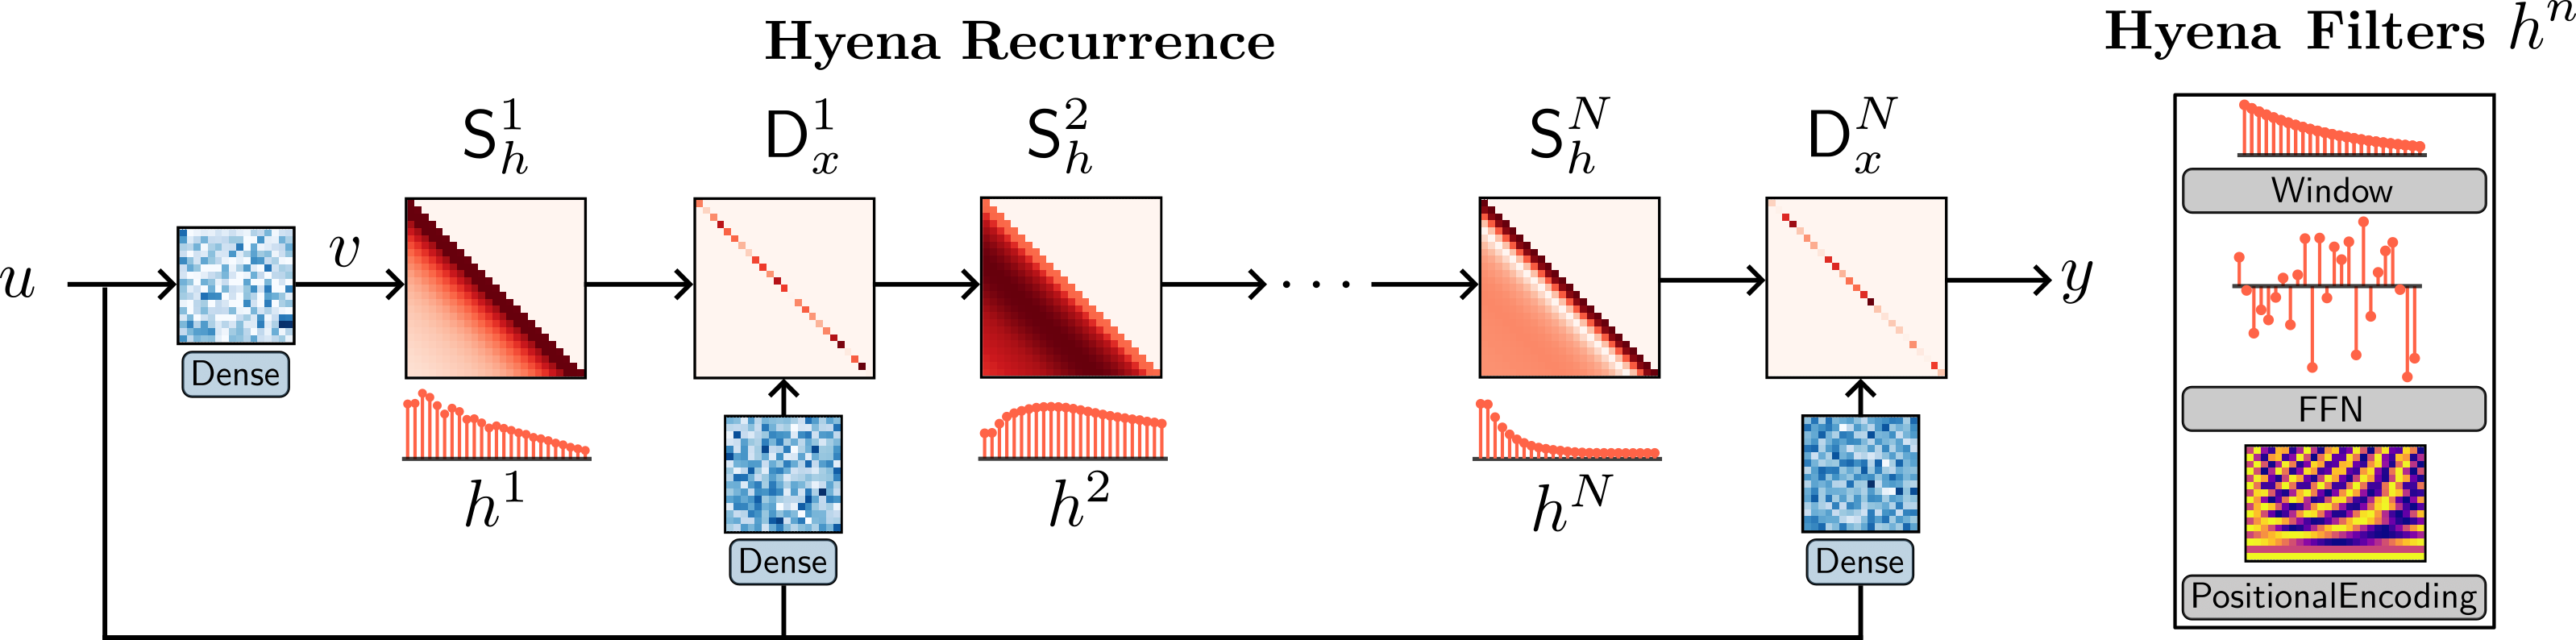
\includegraphics[width=\linewidth]{figures/hyena.png}
    \vspace{-2mm}
    \caption{The ${\sf Hyena}$ operator is defined as a recurrence of two efficient subquadratic primitives: an implicit long convolution $h$ (i.e. {\sf Hyena} filters parameterized by a feed-forward network) and multiplicative element-wise gating of the (projected) input. The depth of the recurrence specifies the size of the operator. {\sf Hyena} can equivalently be expressed as a multiplication with \textit{data-controlled} (conditioned by the input $u$) diagonal matrices $\sD_x$ and Toeplitz matrices $\sS_h$. In addition, {\sf Hyena} exhibits sublinear parameter scaling (in sequence length) and unrestricted context, similar to attention, while having lower time complexity.}
    \label{arch}
\end{figure*}
%

{\centering
\textit{Are there subquadratic operators that can match the quality of attention at scale?}\par}

\vspace{0.5cm}
% 

We obtain a positive answer based on a composition of efficient subquadratic primitives, such as \textit{element-wise multiplication} (gating) and \textit{long convolutions} i.e., convolutions with filter sizes as long as the input. We rely on a set of targeted reasoning tasks, grounded in recent work on \textit{mechanistic interpretability} \citep{elhage2021mathematical,power2022grokking,olsson2022context,zhang2022unveiling} such as recall and induction, to distill three properties of attention correlated with its performance and the quality gap with existing subquadratic approaches: 
%
\begin{itemize}[leftmargin=0.1in]
    \item[$a.$] \textbf{Data control:} Attention implements an expressive \textit{data-controlled} \citep{massaroli2020dissecting} linear operator\footnote{Self-attention can be expressed as $y = \sA(k, q) v$ where $\sA$ is the \textit{attention matrix} conditioned by linear projections $k, q$ of the input and multiplied by $v$, another projection.}, encoding an entire family of linear functions in a single block.
    \item[$b.$] \textbf{Sublinear parameter scaling:} Parameter counts of attention layers are decoupled from sequence length, allowing Transformers to allocate more parameters elsewhere e.g., the \textit{feed-forward neural networks} ({$\sf FFN$s}) between attention layers.
    \item[$c.$] \textbf{Unrestricted context:} For a given input, attention has an unrestricted context i.e., it can approximate dependencies between any two inputs, without arbitrary restrictions such as locality (except in cases using masking such as autoregressive models).
\end{itemize}
%
\paragraph{The ${\sf Hyena}$ hierarchy}
%
Guided by these findings, we introduce the ${\sf Hyena}$ hierarchy, an operator defined by a recurrence of two efficient subquadratic primitives: \textbf{a long convolution and element-wise multiplicative gating} (see Figure \ref{arch}). A specified depth (i.e., number of steps) of the recurrence controls the size of the operator. For short recurrences, existing models are recovered as special cases \citep{mehta2022long,dao2022hungry}. By mapping each step in the ${\sf Hyena}$ recurrence to its corresponding matrix form, we reveal ${\sf Hyena}$ operators to be equivalently defined as a decomposition of a \textit{data-controlled} matrix i.e., a matrix whose entries are functions of the input. Furthermore, we show how ${\sf Hyena}$ operators can be evaluated efficiently without materializing the full matrix, by leveraging fast convolution algorithms \citep{selesnick2017fast}. Empirically, ${\sf Hyena}$ operators are able to significantly shrink the quality gap with attention at scale, reaching similar perplexity and downstream performance with a smaller computational budget (Section \ref{res:lm}) and \textbf{without hybridization} of attention.
%

\paragraph{Narrowing the capabilities gap}
%
The design of {\sf Hyena} is motivated by a quality gap between standard dense attention and alternative subquadratic operators, which we identify by focusing on reasoning tasks correlated with language modeling performance at scale. We extend the suite of basic mechanistic interpretability benchmarks (\textit{induction} and \textit{recall}) with additional tasks that probe how quickly model performance degrades when task complexity increases (e.g. vocabulary size grows). In addition, we investigate the optimal parameterization of long convolutions in ${\sf Hyena}$. In the most challenging settings with hundreds of thousands of tokens, our implicit parameterization scheme improves over other operators leveraging state spaces \citep{gu2021efficiently}, frequency-domain parametrizations \citep{li2020fourier}, or standard convolutions by over $50\%$ accuracy.
%
\paragraph{Scaling in language and vision}
%
Next, we aim to verify whether rankings in our reasoning benchmark suite are predictive of quality at scale. We test ${\sf Hyena}$ on autoregressive language modeling at the sub-billion parameter scale, setting a new state-of-the-art for dense-attention-free architectures in standard datasets ({\sc WikiText103} and {\sc The Pile}) and matching Transformer quality. On the {\sc The Pile} at the $335$M parameter scale, we match Transformer perplexity with a $20\%$ reduction in the total count of \textit{floating point operations} (FLOPs). As an extension, we investigate the generality of ${\sf Hyena}$ operators by testing on large-scale image recognition, replacing attention in the Vision Transformer (ViT) \citep{dosovitskiy2020image}. In image classification, ${\sf Hyena}$ is able to match attention in accuracy when training on ImageNet-1k from scratch.
%
\paragraph{Toward much longer context}
%
Finally, we benchmark the efficiency of ${\sf Hyena}$ on long sequences. We measure $5$x speedups over dense self-attention at length $8192$ -- $2$x over highly optimized FlashAttention\footnote{FlashAttention is already 2-4x faster than a standard attention implementation in PyTorch.} \citep{dao2022flashattention} -- and $100$x speedup over FlashAttention at sequence lengths of $64$k, where standard attention implementation in PyTorch runs out of memory. 
\label{sec:introduction}
%-------------------------------------------------------------------------------

%-------------------------------------------------------------------------------
\section{Related work}
\section{Related Work}
\subsection{Diffusion Model}
%
In the realm of generative models, diffusion models \cite{ho2020denoising, sohl2015deep} have become foundational due to their exceptional ability to produce high-quality and diverse outputs. Initially developed with the U-Net architecture, these models have demonstrated impressive performance in image and video generation \cite{ramesh2022hierarchical, rombach2022high, ho2022video, saharia2022photorealistic, wei2024dreamvideo, wei2024dreamvideo2, wang2023modelscope, chen2023videocrafter1, chen2024videocrafter2}. 
%

However, the scalability of U-Net-based diffusion models is inherently constrained, posing challenges for applications requiring larger model capacities for enhanced performance. To address this limitation, Diffusion transformers (DiT) \cite{peebles2023scalable} represent a significant advancement. By utilizing the scalable architecture of transformers \cite{vaswani2017attention}, DiT provides an effective means to increase model capacity.
%
A notable achievement in this field is the advancement in generating long videos through the large-scale training of Sora \cite{Sora}, which employs a transformer-based Diffusion architecture for comprehensive simulations of the physical world. This underscores the considerable impact of scaling transformer-based Diffusion models.
%
An increasing number of studies have adopted the Diffusion transformer as the noise estimation network~\cite{chen2023pixart, chen2024pixart, Open-Sora, Open-Sora-Plan, ma2024latte, yang2024cogvideox}.

\subsection{Diffusion Model Acceleration}
%
Despite the notable performance of Diffusion models in image and video synthesis, their significant inference costs hinder practical applications. Efforts to accelerate Diffusion model inference fall into two primary categories. First, techniques such as DDIM~\cite{song2020denoising} allow for fewer sampling steps without sacrificing quality. Additional research has focused on efficient ODE or SDE solvers~\cite{song2019generative, jolicoeur2021gotta, lu2022dpm, karras2022elucidating, lu2022dpm++}, using pseudo numerical methods for faster sampling. Second, approaches include distillation~\cite{salimans2022progressive, wang2023videolcm}, quantization~\cite{li2024q, he2024ptqd, so2024temporal, shang2023post}, and distributed inference~\cite{li2024distrifusion} are employed to reduce the workload and inference time.  

However, these methods often demand additional resources for fine-tuning or optimization. Some training-free approaches~\cite{bolya2023token, wang2024attention} streamline the sampling process by reducing input tokens, thereby eliminating redundancy in image synthesis. Other methods reuse intermediate features between successive timesteps to avoid redundant computations~\cite{wimbauer2024cache, so2023frdiff, zhang2024cross}. DeepCache~\cite{xu2018deepcache} and Faster Diffusion~\cite{li2023faster} utilize feature caching to modify the UNet Diffusion, thus enhancing acceleration. FORA~\cite{selvaraju2024fora} and $\triangle$-DiT~\cite{chen2024delta} adapts this mechanism to DiT by caching residuals between attention layers. PAB~\cite{zhao2024real} caches and broadcasts intermediate features at various timestep intervals based on different attention block characteristics for video synthesis. While these methods have improved Diffusion efficiency, enhancements for DiT in visual synthesis remain limited.
\label{sec:related_work}
%-------------------------------------------------------------------------------

%-------------------------------------------------------------------------------
\section{Fuzzy trap sequences}
\section{Method}
\label{sec:method}

\subsection{Practical choice of diffusion paradigm}
\label{subsec:practical_dwm}

Building on the background provided in Section \ref{sec:framework}, we now introduce \textsc{diamond} as a practical realization of a diffusion-based world model. In particular, we now define the drift and diffusion coefficients $\mathbf{f}$ and $g$ introduced in Section \ref{subsec:diffusion}, corresponding to a particular choice of diffusion paradigm. While \textsc{ddpm} \citep{ho2020DDPM} is an example of one such choice (as described in Appendix \ref{app:ddpm}) and would historically be the natural candidate, we instead build upon the \textsc{edm} formulation proposed in \citet{karras2022elucidating}. The practical implications of this choice are discussed in Section \ref{subsec:diffusion_choice}. In what follows, we describe how we adapt \textsc{edm} to build our diffusion-based world model.

We consider the perturbation kernel $p^{0\tau}(\x_{t+1}^\tau \mid \x_{t+1}^0) = \mathcal{N}(\x_{t+1}^\tau; \x_{t+1}^0, \sigma^2(\tau) \mathbf{I})$, where $\sigma(\tau)$ is a real-valued function of diffusion time called the noise schedule. This corresponds to setting the drift and diffusion coefficients to $\mathbf{f}(\x, \tau) = \mathbf{0}$ (affine) and $g(\tau) = \sqrt{2 \dot \sigma(\tau) \sigma(\tau)}$.

We use the network preconditioning introduced by \citet{karras2022elucidating} and so parameterize $\mathbf{D}_\theta$ in Equation \ref{eq:denoising_sm_conditional} as the weighted sum of the noised observation and the prediction of a neural network $\mathbf{F}_\theta$,
\begin{equation}
\label{eq:karras_wrappers} 
    \mathbf{D}_\theta(\x_{t+1}^\tau, y_t^\tau) = c_\text{skip}^\tau \; \x_{t+1}^\tau + c_\text{out}^\tau \; \mathbf{F}_\theta \big( c_\text{in}^\tau \; \x_{t+1}^\tau, y_t^\tau \big),
\end{equation}
where for brevity we define $y_t^\tau \coloneqq (c_\text{noise}^\tau, \x^0_{\le t}, a_{\le t})$ to include all conditioning variables.

The preconditioners $c_\text{in}^\tau$ and $c_\text{out}^\tau$ are selected to keep the network's input and output at unit variance for any noise level $\sigma(\tau)$, $c_\text{noise}^\tau$ is an empirical transformation of the noise level, and $c_\text{skip}^\tau$ is given in terms of $\sigma(\tau)$ and the standard deviation of the data distribution $\sigma_\text{data}$, as $c_{skip}^\tau = \sigma_{data}^2/(\sigma_{data}^2 + \sigma^2(\tau))$. These preconditioners are fully described in Appendix \ref{appendix:karras_conditioners}.

Combining Equations \ref{eq:denoising_sm_conditional} and \ref{eq:karras_wrappers} provides insight into the training objective of $\mathbf{F}_\theta$,
\begin{align}
\label{eq:effective_obj}
\mathcal{L}(\theta)  = \bbe \Big[ \Vert 
\underbrace{\mathbf{F}_\theta \big( c_\text{in}^\tau \x_{t+1}^\tau, y_t^\tau \big)}_\text{Network prediction} - 
\underbrace{\frac{1}{c_\text{out}^\tau} \big( \x_{t+1}^0 - c_\text{skip}^\tau \x_{t+1}^\tau\big)}_\text{Network training target}
\Vert^2 \Big].
\end{align}
The network training target adaptively mixes signal and noise depending on the degradation level $\sigma(\tau)$.
When $\sigma(\tau) \gg \sigma_\text{data}$, we have $c_\text{skip}^\tau \to 0$, and the training target for $\mathbf{F}_\theta$ is dominated by the clean signal $\x_{t+1}^0$. Conversely, when the noise level is low, $\sigma(\tau) \to 0$, we have $c_\text{skip}^\tau \to 1$, and the target becomes the difference between the clean and the perturbed signal, i.e. the added Gaussian noise. Intuitively, this prevents the training objective to become trivial in the low-noise regime. In practice, this objective is high variance at the extremes of the noise schedule, so \citet{karras2022elucidating} sample the noise level $\sigma(\tau)$ from an empirically chosen log-normal distribution in order to concentrate the training around medium-noise regions, as described in Appendix \ref{appendix:karras_conditioners}.

We use a standard U-Net 2D for the vector field $\mathbf{F}_\theta$ \citep{ronneberger2015unet}, and we keep a buffer of $L$ past observations and actions that we use to condition the model. We concatenate these past observations to the next noisy observation channel-wise, and we input actions through adaptive group normalization layers \citep{adagn} in the residual blocks \citep{He2015} of the U-Net.

As discussed in Section \ref{subsec:dwm_training} and Appendix \ref{appendix:sampling}, there are many possible sampling methods to generate the next observation from the trained diffusion model. While our codebase supports a variety of sampling schemes, we found Euler's method to be effective without incurring the cost of additional NFE required by higher order samplers, or the unnecessary complexity of stochastic sampling.

\subsection{Reinforcement learning in imagination}
\label{subsec:rl}

Given the diffusion model from Section \ref{subsec:practical_dwm}, we now complete our world model with a reward and termination model, required for training an RL agent in imagination. Since estimating the reward and termination are scalar prediction problems, we use a separate model $R_\psi$ consisting of standard \textsc{cnn} \citep{cnn_lecun,He2015} and \textsc{lstm} \citep{lstm,Gers2000} layers to handle partial observability. The RL agent involves an actor-critic network parameterized by a shared \textsc{cnn-lstm} with policy and value heads. The policy $\pi_\phi$ is trained with \textsc{reinforce} with a value baseline, and we use a Bellman error with $\lambda$-returns to train the value network $V_\phi$, similar to \citet{iris2023}. We train the agent entirely in imagination as described in Section \ref{subsec:pomdp_and_wm}. The agent only interacts with the real environment for data collection. After each collection stage, the current world model is updated by training on all data collected so far. Then, the agent is trained with RL in the updated world model environment, and these steps are repeated. This procedure is detailed in Algorithm \ref{alg:diamond}, and is similar to \citet{kaiser2019atari100k,hafner2020dream,iris2023}. We provide architecture details, hyperparameters, and RL objectives in Appendices \ref{app:architectures}, \ref{app:hyperparams}, \ref{appendix:rl_actor_critic}, respectively.

\label{sec:method}
%-------------------------------------------------------------------------------

%-------------------------------------------------------------------------------
\section{Experimental Setup}
\textbf{Models.} As target model \textit{LM} we use the pretrained 1.3B CroissantLLM~\cite{faysse2024croissantllm}, which we fine-tune on documents containing fuzzy trap sequences. As reference model $\textit{LM}_{\text{ref}}$, we use the pretrained LLaMA-2 7B~\cite{touvron2023llama2} to generate the synthetic reference trap sequences. Finally, as masked language model $\textit{MLM}$, we use RoBERTa~\cite{liu2019roberta} to generate the fuzzy duplicates.

\textbf{Fuzzy trap sequences.} We generate $100$ reference trap sequences using $\textit{LM}_{\text{ref}}$. We specifically control for the sequence length ($L_{\text{ref}}(X_{\text{ref}}) = 100$), and perplexity (between 90 and 100) to minimize variance in memorization, as previous works have shown length and perplexity to correlate with memorization~\cite{meeus2024copyright, carlini2022quantifying}. Unless stated otherwise, we use $k=50$ when selecting top $k$ tokens predicted by masked language model $\textit{MLM}$. For number of replacements we consider $R=\{1, 2, 4, 8, 16, 32\}$.

\textbf{Data.} We inject fuzzy trap sequences in a collection of books available in the public domain. We use the open-source library~\cite{kpullygutenberg} to collect $100$ books made available under a permissive license on Project Gutenberg~\cite{projectgutenberg} but have not been included in the training dataset of CroissantLLM~\cite{faysse2024croissantllm}. The books we selected contain $8.7$M tokens in total (tokenized with CroissantLLM tokenizer). For each of the $100$ reference trap sequences, we inject the $n_{\text{dup}}=10$ fuzzy trap sequences at random into one book and use this collection of modified books as dataset for fine-tuning. 

\textbf{Fine-tuning.} In all of our experiments we fine-tune CroissantLLM~\cite{faysse2024croissantllm} on the $100$ modified books for $1$ epoch. We use its maximum sequence length of $2048$ tokens, a batch size of $6$ and optimizer Adam with constant learning rate \num{3e-6} and weight decay of $0.01$. Unsurprisingly, we find that the extent to which the target model \textit{LM} memorizes the trap sequences at the fixed number of training steps, heavily depends on the learning rate. We elaborate on this in Sec~\ref{section:ablations} and throughout the rest of the experiments consider the learning rate fixed to \num{3e-6}. We argue, however, that the \emph{absolute} extent of memorization does not impact our findings, as we here study how fuzzy trap sequences are memorized \emph{relative} to exact duplication of trap sequences, which have been shown by Meeus et al.~\cite{meeus2024copyright} to be memorized in a real-world scenario. Fine-tuning one model on $100$ trap-injected books took roughly 2 GPU-hours on A100 NVIDIA GPUs.

\textbf{Membership Inference Attack (MIA).} To measure the memorization of the fuzzy trap sequences, we instantiate a sequence-level MIA to infer whether $X_{\text{ref}}$ has been seen by the target model \textit{LM}. For this, we generate $100$ new reference trap sequences, which we do not include in the training dataset and thus consider as \emph{non-members}. We consider the $100$ reference trap sequences that are included in the training dataset as \emph{members}. As MIA methodology, we use the \textit{Ratio} attack~\cite{carlini2021extracting}. For each $X_{\text{ref}}$, either \emph{member} or \emph{non-member}, we compute the target model loss divided by the loss computed using the reference model, which we call \emph{membership score} $\alpha(X_{\text{ref}}) = \mathcal{L}_{\textit{LM}}(X_{\text{ref}}) / \mathcal{L}_{\textit{LM}_{\text{ref}}}(X_{\text{ref}})$. We then use $\alpha(X_{\text{ref}})$ to compute the ROC AUC for the binary membership prediction task and use the AUC to measure to what extent the fully trained target model \textit{LM} memorizes the trap sequences. We compute the AUC on $25$ bootstrapped subsets of members and non-members and report both the mean and standard deviation across all results~\cite{bertail2008bootstrapping}. %\todo{See Q.7 in the checklist: we need to explain more on the error bars}

\textbf{Baselines.} The primary goal of this paper is to quantify how fuzzy trap sequences are memorized compared to exact duplication. For 10 fuzzy trap sequences $\{X_\text{ref}, X_2, X_3, \ldots X_{n_{\text{dup}}}\}$, where each $X_i$ has $R$ tokens replaced compared to $X_{\text{ref}}$, we consider the following baselines. As an upper bound, we consider the exact repetition of the reference trap sequence $X_{\text{ref}}$ for $n_{\text{dup}}=10$ times. As a lower bound we consider a single injection of the reference trap sequence, i.e. $n_{\text{dup}}=1$. 

\textbf{Reproducibility.} We will share the code to reproduce our results in the camera-ready version.
\label{sec:experimental_setup}
%-------------------------------------------------------------------------------


%-------------------------------------------------------------------------------
\section{LLMs have mosaic memory}
\begin{table*}[ht]
    \centering
    \begin{tabular}{ccc|cc}
    \toprule
         & \multicolumn{2}{c}{AUC} & \multicolumn{2}{c}{$C_\text{max}$} \\
        $R$ & Random & Even & Random & Even\\
        \midrule
        $1$ & $0.893 \pm 0.022$ & $0.903 \pm 0.022$ & $91.43 \pm 1.60$ & $91.01 \pm 1.80$ \\ 
        \cmidrule{1-5}
        $2$ & $0.891 \pm 0.026$ & $0.890 \pm 0.025$ & $79.97 \pm 1.35$ & $73.46 \pm 1.86$ \\ 
        \cmidrule{1-5}
        $4$ & $0.869 \pm 0.022$ & $0.861 \pm 0.024$ & $61.40 \pm 1.77$ & $41.26 \pm 0.82$ \\ 
         \cmidrule{1-5}
        $8$ & $0.840 \pm 0.027$ & $0.834 \pm 0.029$ & $42.39 \pm 1.47$ & $21.51 \pm 0.51$ \\  
         \cmidrule{1-5}
        $16$ & $0.783 \pm 0.032$ & $0.754 \pm 0.032$ & $25.90 \pm 0.70$ & $10.90 \pm 0.23$ \\ 
         \cmidrule{1-5}
        $32$ & $0.682 \pm 0.022$ & $0.646 \pm 0.041$ & $13.54 \pm 0.42$ & $5.89 \pm 0.13$ \\ 
         \bottomrule
    \end{tabular}
    \caption{AUC and $C_\text{max}$ (mean and standard deviation) for \emph{Random} and \emph{Even} replacement position distribution.}
    \label{tab:uniform_vs_random_distr}
\end{table*}

Fig.~\ref{fig:auc_vs_r_main} shows how the AUC varies for increasing number of replacements $R$ made to the fuzzy trap sequences. We find that the AUC only drops slightly for smaller values of replacements $R$. For $R=4$, when $n_{\text{dup}}=10$ fuzzy trap sequences are injected, the mean AUC only drops from $0.90$ to $0.87$. Even at $R=32$, when we replace roughly one third of all tokens in the sequence, the mean AUC is $0.68$ and remains significantly higher than a single repetition $n_{\text{dup}}=1$ with a mean AUC of $0.59$. This demonstrates the mosaic memory in the target LLM, i.e. the overlapping fragments of multiple, slightly different sequences contribute to the memorization of the reference trap sequence.

\subsection{Replacement position distribution.} \label{section:spread_replacements}

We now aim to further reduce the chances of fuzzy trap sequences being removed by deduplication, and ensure that token replacements are evenly spread across the sequence. Above, we have uniformly at random sampled tokens to be replaced across fuzzy duplicates. Here, we instantiate the exact same setup, but we split the tokenized reference trap sequence using the MLM tokenizer: $T_{\text{MLM}}(X_{\text{ref}}) = \{t_1,\ldots,t_N\}$ in $R$ equally-sized chunks of size $\lceil\frac{N}{R}\rceil$. We then replace exactly one (selected uniformly at random) token for every chunk. Below we refer to this strategy as \emph{Even}, and to the previously used strategy as \emph{Random}.

We also compute the length of subsequences repeated exactly within clusters of fuzzy duplicates, simulating a sequence-level deduplication algorithm. We define $C_\text{max}$ as the maximum length (in tokens) of a substring shared by at least two fuzzy duplicate sequences within a cluster. We report the mean $C_\text{max}$ across 100 clusters used in our experiments.

Table~\ref{tab:uniform_vs_random_distr} shows that for smaller values of $R$ (up to $R=8$) the AUC for \textit{randomly} and \textit{evenly} distributed token replacements remains highly similar. For larger values of $R$ ($R \geq 16$), the impact of uniform spreading becomes more apparent, leading to a slightly lower AUC. At the same time, $C_\text{max}$ is significantly lower for the evenly distributed token replacements, with the impact more pronounced at higher values of $R$. This demonstrates how a reasonable number of token replacements ($R=4$ or $R=8$) would evade even the sequence-level deduplication with the most aggressive threshold (e.g. $50$ tokens), while retaining significant memorization.

\subsection{MIAs adapted to fuzzy trap sequences.} \label{section:adapted_mia}

So far we have used the unmodified \textit{Ratio} attack~\cite{carlini2021extracting} to infer whether the reference trap sequence has been seen by the target model. Specifically, we compute a single $\alpha(X_{\text{ref}}) = \alpha(X_1)$ for each trap sequence, and do not utilize our knowledge of the fuzzy counterparts $\{X_i \mid i=2 \ldots n_{\text{dup}}\}$. To evaluate whether this could further improve detectability, we now compute the membership score for each of the fuzzy trap sequences, i.e. $\{\alpha(X_i) \mid i=1 \ldots n_{\text{dup}}\}$, and aggregate the membership scores with aggregation function $\mathcal{A}(\cdot)$, i.e. $\alpha_{\mathcal{A}}(X_{\text{ref}}) = \mathcal{A}\left( \{\alpha(X_i) \mid i=1 \ldots n_{\text{dup}}\}\right)$. We then compute $\alpha_{\mathcal{A}}(X_{\text{ref}})$ for each reference trap sequence. We compute AUC on a balanced set of \emph{members} and \emph{non-members}, and so generate fuzzy trap sequences for all non-member sequences too. As aggregation function $\mathcal{A}$ we consider the mean, median, minimum and maximum. We report the MIA AUC for all aggregation functions, and for $R=\{2, 8, 32\}$ for models trained in the main experiment (Fig.~\ref{fig:auc_vs_r_main}). As a baseline, we also provide the previously used MIA based on the reference trap sequence $\alpha(X_{\text{ref}})$ alone.

 Table~\ref{tab:custom_MIA} shows that aggregating the membership score on all fuzzy trap sequences $\alpha_{\mathcal{A}}(X_{\text{ref}})$ does not provide substantial benefits compared to the baseline. We attribute this to the fact that all fuzzy trap sequences $X_i$ only differ from $X_{\text{ref}}$ by $R$ replacements, and therefore the target model loss computed on the reference trap sequence likely captures an aggregation across its fuzzy trap sequences already.

\begin{table*}[ht]
    \centering
    \begin{tabular}{cccc}
    \toprule
         & \multicolumn{3}{c}{AUC} \\
        Aggregation $\mathcal{A}$ & $R=2$ & $R=8$ & $R=32$ \\
        \midrule
        $\alpha(X_{\text{ref}})$ - no aggregation & $0.891 \pm 0.026$ & $0.840 \pm 0.027$ & $0.682 \pm 0.022$ \\ 
         \midrule
         \midrule
        Mean & $0.870 \pm 0.021$ & $0.828 \pm 0.029$ & $0.683 \pm 0.026$ \\ 
         \cmidrule{1-4}
        Median & $0.869 \pm 0.028$ & $0.824 \pm 0.030$ & $0.692 \pm 0.039$ \\  
         \cmidrule{1-4}
        Minimum & $0.881 \pm 0.021$ & $0.823 \pm 0.030$ & $0.624 \pm 0.040$  \\ 
         \cmidrule{1-4}
        Maximum & $0.879 \pm 0.030$ & $0.821 \pm 0.034$ & $0.679 \pm 0.041$  \\ 
         \bottomrule
    \end{tabular}
    \label{tab:custom_MIA}
    \caption{AUC (mean and standard deviation) for MIA methodologies adapted to fuzzy trap sequences.}
\end{table*}



\subsection{Ablation studies.} \label{section:ablations}

\textbf{Token replacement hyperparameters.} We here explore whether the semantic coherence of fuzzy trap sequences $X_i$ affect memorization. For this, we vary the value $k$ when sampling replacements from the top-$k$ tokens predicted by the MLM when a fixed number $R=8$ of replacements are made (see Sec.~\ref{sec:method_gen_fuzzy}). Recall that thus far we only considered $k=50$ and that for $k=|\mathcal{V}_{\text{MLM}}|$ -which is $50,000$ for RoBERTa~\cite{liu2019roberta}-, we effectively randomly sample a token from the entire MLM vocabulary $\mathcal{V}_{\text{MLM}}$. In addition to sampling uniformly from the top $k$ tokens, we also consider sampling directly from the full probability distribution predicted by the MLM (\textit{Sample directly}).

Fig.~\ref{fig:robustness}(a) shows that the AUC decreases as $k$ increases. We find $k$ and AUC to be strongly correlated with a Spearman coefficient of $-0.47$ and a p-value of \num{4e-11}, suggesting that semantic coherence is important for mosaic memorization. Further, Fig.~\ref{fig:robustness}(b) compares the AUC for $k=50$ and $k=|\mathcal{V}_{\text{MLM}}|$ for increasing values of $R$. For a smaller amount of replacements $R$, the AUC for $k=50$ and random token replacement remains very similar. For larger values of $R$ the mean estimations start to diverge, yet with no statistically significant difference.

\textbf{Impact of learning rate.} We here show, that the key outcome of our experiments - the \emph{relative} memorization of fuzzy duplicates compared to exact duplicates holds regardless of the \emph{absolute} level of memorization. At a fixed number of training steps we can control the baseline memorization with varying learning rate. So far in previous experiments, we have considered a fixed learning rate of $\num{3e-6}$. Fig.~\ref{fig:robustness} (b) shows how for increasing learning rate the AUC for fuzzy trap sequences remains consistently slightly lower than the upper bound ($n_{dup} = 10$), while remaining significantly higher than the lower bound ($n_{dup} = 1$). This suggests that fuzzy trap sequences are also memorized in lower and higher memorization regimes. 

\begin{figure*}[ht]
\centering
\subfigure{
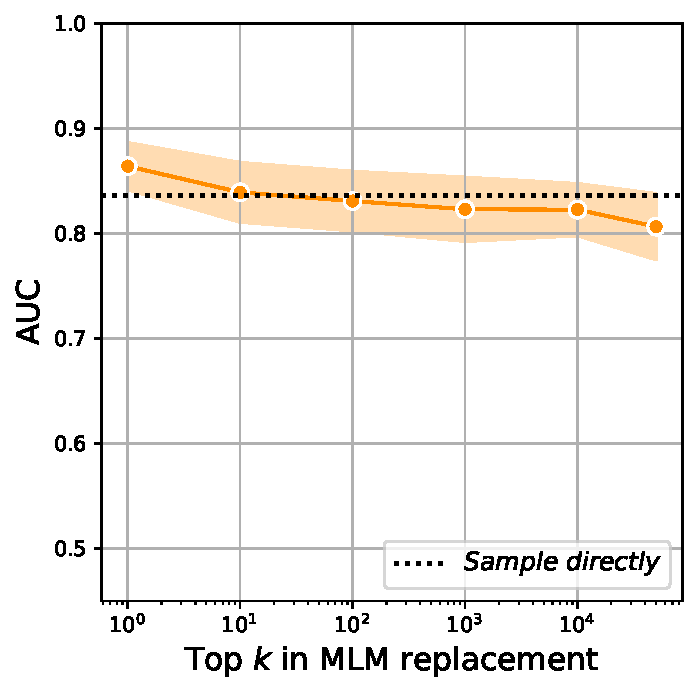
\includegraphics[width=0.3\linewidth]{figures/vary_k.pdf}
}
\subfigure{
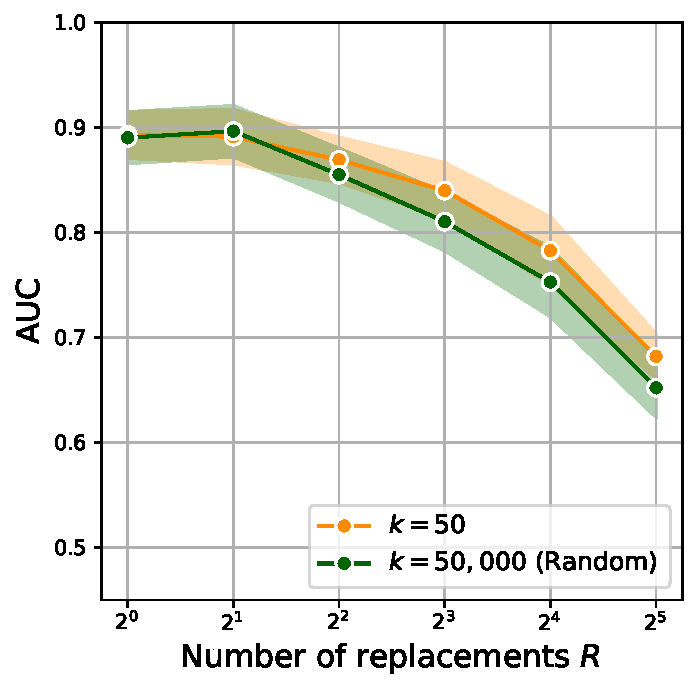
\includegraphics[width=0.3\linewidth]{figures/AUC_vs_R_both_strategies.pdf}
}
\subfigure{
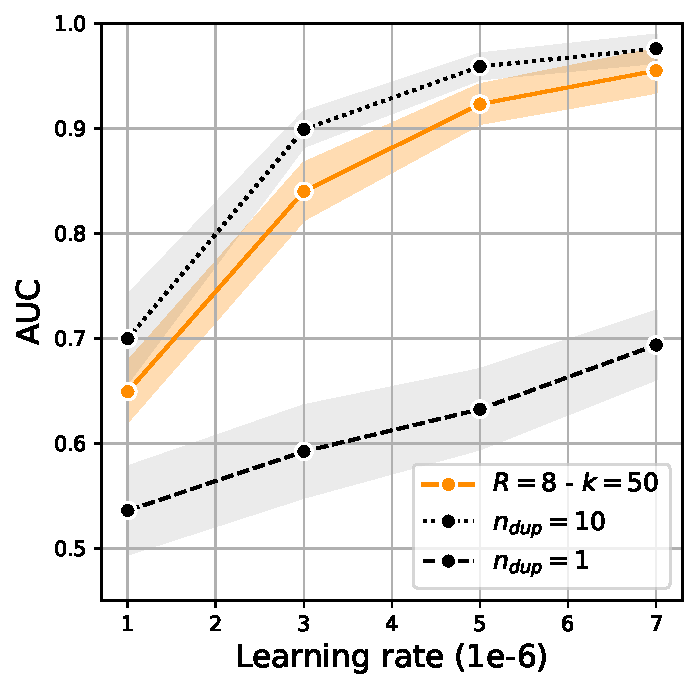
\includegraphics[width=0.3\linewidth]{figures/vary_lr.pdf}
}

    \caption{\textbf{Ablation.} MIA AUC (mean and standard deviation) for fuzzy trap sequences for (a) varying $k$ for $R=8$, (b) $k=50$ and $k=50,000$ across $R$ and (c) varying learning rate used in fine-tuning.} 
\label{fig:robustness}
\end{figure*} 

\label{sec:experiments}
%-------------------------------------------------------------------------------

%-------------------------------------------------------------------------------
\section{Implications for measuring post-hoc LLM memorization.}
\begin{figure*}[ht]
\centering
\subfigure{
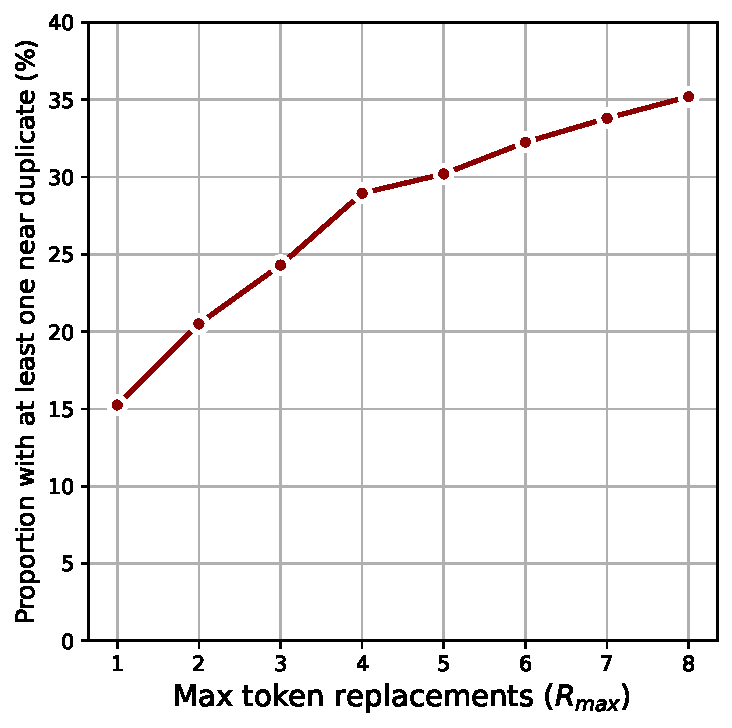
\includegraphics[width=0.4\linewidth]{figures/near_duplicates_proportion.pdf}
}
\subfigure{
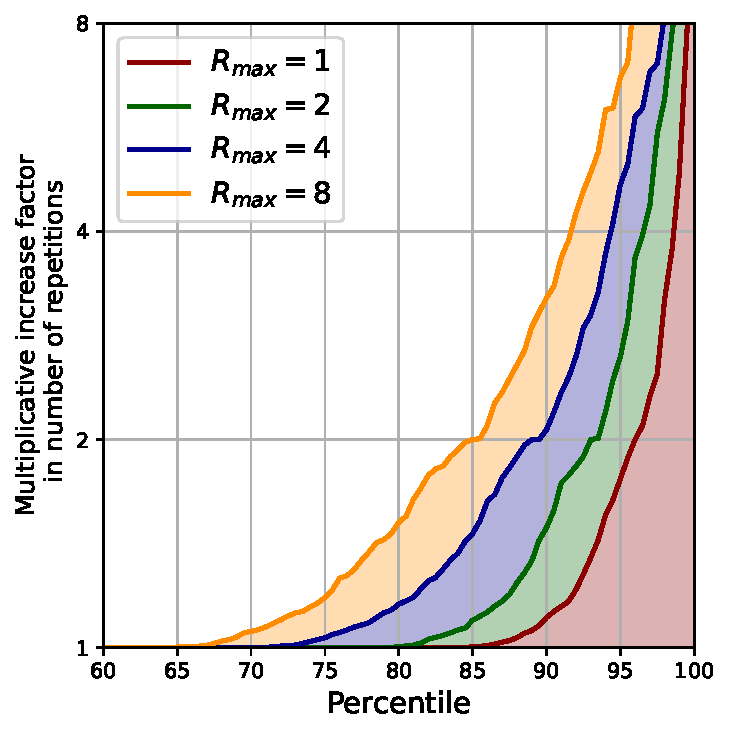
\includegraphics[width=0.4\linewidth]{figures/near_duplicates_percentiles.pdf}
}
\caption{\textbf{Fuzzy duplicate sequences in The Pile.} (a) Proportion of sequences with at least one fuzzy duplicate given the maximum threshold $R_\text{max}$ (b) An increase in total number of repetitions if accounting for fuzzy duplicates given the maximum threshold $R_\text{max}$.}
\label{fig:near_dups}
\end{figure*}


Prior work on memorization in LLMs often relies on the natural presence of the duplicated sequences in large text datasets~\cite{carlini2021extracting,carlini2022quantifying,kandpal2022deduplicating, ippolito2022preventing}. For instance, seminal work by Carlini et al.~\cite{carlini2022quantifying} identifies sequences repeated multiple times in The Pile~\cite{pile}, and uses this to study the relationship between the number of repetitions and memorization. Kandpal et al.~\cite{kandpal2022deduplicating} adopts a similar approach with C4~\cite{2019t5} and OpenWebText~\cite{Gokaslan2019OpenWeb}.

We argue that relying on naturally occurring duplicates might overestimate the impact of exact duplication on memorization. Instead, some memorization could be attributed to fuzzy duplicates. Any memorization study using the set of exact duplicates found in a large text dataset is susceptible to the confounding factor from the presence of fuzzy duplicates. As we show below, the number of fuzzy duplicates tend to be distributed in a highly non-uniform fashion, likely introducing bias when studying memorization.

To verify this, we here re-create the set of sequences duplicated in The Pile considered by prior work. We use the code provided by Lee et al.~\cite{lee2022deduplicating}\footnote{Distributed under Apache License 2.0.} to build a suffix array and identify sequences occurring at least twice in the dataset. We consider sequences of 100 BPE (GPT-2) tokens~\cite{radford2019language}. As the original The Pile has been taken down due to copyright violations in some of its subsets, we study the non-copyrighted version of The Pile~\cite{pile_uncopyrighted}, which covers roughly 80\% of the original data\footnote{The rest of The Pile is distributed under a range of permissive licences.}. While this affects the absolute counts of exact and fuzzy duplicates, we effectively report the lower bound on both counts, which allows us to study their relative prevalence in large datasets. Data processing took us $\sim96$ hours on a machine with 96 CPUs, 500GB of RAM and 5TB of available disk space.

Following the approach proposed by Carlini et al.~\cite{carlini2022quantifying}, we group duplicate sequences into buckets by the number of exact repetitions, where the $n$-th bucket contains sequences repeated between $2^{n/4} \leq n_{dup} < 2^{(n+1)/4}$ times in the dataset. We consider $n \in [20, 40)$, thus covering sequences repeated between $32$ and $1024$ times. We then sample $100$ random sequences from each bucket (2000 sequences overall) and search for their fuzzy duplicates. As in the experiments above, we define a fuzzy duplicate as a sequence of the same length with up to a certain number of tokens ($R_\text{max}$) replaced between the two sequences (we consider $R_\text{max} \leq 8$). Note that the notion of the number of tokens replaced between two sequences of the same length is equivalent to the Hamming distance - we here adopt the former for consistency.  
For computational reasons, we only look for fuzzy duplicates among sequences identified as duplicates themselves, i.e. repeated in the original dataset at least twice. Our fuzzy duplicate counts, therefore, only provide a lower bound estimation of the total number of fuzzy duplicates for a given sequence.

Our results show that a significant proportion of sequences duplicated in The Pile have additional fuzzy duplicates in the dataset. Fig.~\ref{fig:near_dups}(a) shows that almost 15\% and 30\% of sequences have at least one fuzzy duplicate with only a $R_\text{max}=1$ and $R_\text{max}=4$ token replacements respectively (out of a 100 tokens in the sequence). Strikingly, Fig.~\ref{fig:near_dups}(b) shows that for 10\% of all duplicate sequences, the number of fuzzy duplicates ($R_\text{max}=4$) is larger than the number of exact repetitions. For instance, 10\% of all sequences repeated $32$ times in The Pile have more than $32$ additional fuzzy duplicates. This data suggests that using naturally occurring duplicates to study memorization is prone to unforeseen confounding factors, such as the presence of fuzzy duplicates illustrated above.
\label{sec:naturally_occuring}
%-------------------------------------------------------------------------------

%-------------------------------------------------------------------------------
\section{Discussion and Future Work}

\textbf{Feasibility of copyright traps.} We here focus on addressing one core limitation of implementing copyright traps in practice: the potential accidental removal during training data deduplication~\cite{lee2022deduplicating,kudugunta2024madlad,penedo2023refinedweb}. We now consider other potential limitations. First, traps might be affected by quality filters. For instance, prior work has implemented filtering based on language ~\cite{penedo2023refinedweb,soldaini2024dolma}, certain heuristics (e.g. removing sequences with a high ratio of special characters)~\cite{kudugunta2024madlad,rae2021scaling,laurenccon2022bigscience} and perplexity~\cite{wenzek2019ccnet}. We here argue that trap sequences are designed to resemble human-generated text, and preprocessing techniques sufficiently aggressive to remove traps are also likely to hurt model utility. While we do not believe any of the current filtering techniques to affect fuzzy copyright traps, we leave for future work to explore if the wide variety of filtering mechanisms~\cite{albalak2024survey} could remove trap sequences. Second, (fuzzy) trap sequences likely impact the readability of the original content. However, as also argued when introduced~\cite{meeus2024copyright,wei2024proving}, traps injected in web-based publications can be made invisible to a human reader yet picked up by a scraper. Lastly, we acknowledge that traps can potentially be removed by an informed and motivated adversary with techniques targeted specifically at trap sequences.

\textbf{Privacy and confidentiality.} Our findings highlight new challenges in addressing privacy issues associated with LLMs. Sec.~\ref{sec:naturally_occuring} elaborates on challenges for post-hoc studies on LLM memorization. Further, we argue that deduplication does not necessarily eliminate privacy risks in LLMs~\cite{kandpal2022deduplicating}, as some duplicate sequences also tend to have many fuzzy duplicates in the same dataset. Thus, even the more aggressive sequence-level deduplication techniques would not be able to remove fuzzy duplicates and leave the data prone to memorization. 

\textbf{Potential for misuse.} With the injection of carefully designed fuzzy sequences and their memorization in a target LLM becoming feasible, we also acknowledge the potential misuse of this technology. For instance, malicious actors could leverage similar techniques to inject targeted misinformation into public content, which could potentially be propagated through LLMs deployed in practice. Future work could study whether our findings on memorization apply to the spread of misinformation and investigate potential mitigation strategies.  


\label{sec:discussion}
%-------------------------------------------------------------------------------

%-------------------------------------------------------------------------------
\section{Conclusion}

Copyright traps are unique synthetic sequences injected into original content, enabling its detectability in LLM training. However, traps rely on exact duplication across the content -up to 1,000 times-, making them vulnerable to accidental removal as part of commonly deployed deduplication strategies. We here propose \emph{fuzzy} copyright traps. By replacing a small amount of tokens across duplication, traps become increasingly unlikely to be removed - while we find their detectability to only decrease slightly. In our setup, fuzzy trap sequences with $4$ token replacements in a sequence of $100$ tokens, the mean MIA AUC only drops from $0.90$ to $0.87$ - while now being highly unlikely to be removed by deduplication techniques. 

The fact that fuzzy duplicates are memorized to a similar extent as exact duplicates has implications for LLM memorization and confidentiality. First, we find that in a dataset widely used to train LLMs and study post-hoc memorization, The Pile, many duplicated sequences also have a significant amount of fuzzy duplicates - almost 30\% have at least one, but potentially many more, fuzzy duplicates with as little as 4 mismatched tokens.
We expect this to be a common feature of large text datasets, and to present a major confounding factor in studying memorization using duplicate sequences from such datasets.
Further, our findings highlight additional challenges in training LLMs on private or confidential data. We show that techniques like data deduplication might not be sufficient to eliminate risks of information leakage.
\label{sec:conclusion}
%-------------------------------------------------------------------------------

\bibliographystyle{plain}
\bibliography{bibliography.bib}

\onecolumn
\newpage
\appendix

\section{Characterizing fuzzy trap sequences}
\label{app:fuzzy_trap_sequences}
In Sec.~\ref{sec:method_gen_fuzzy}, we describe the generation of fuzzy trap sequences from a reference trap sequence $(X_{\text{ref}})$. First, we tokenize the reference trap sequence using the tokenizer of a masked language model MLM, resulting in $T_{\text{MLM}}(X_{\text{ref}}) = \{t_1,\ldots,t_N\}$. Due to the different tokenization of $T_{\text{ref}}$ and $T_{\text{MLM}}$, $N$ differs from $L_{\text{ref}}$. Fig~\ref{fig:tokens_ppl} (a) shows how the $N=|T_{\text{MLM}}(X_{\text{ref}})|$ is distributed for $100$ reference trap sequences - which all have $L_{\text{ref}}=100$. 

Next, to generate fuzzy trap sequences, we replace $R$ tokens by sampling from the top $k$ tokens predicted by the MLM. For smaller values of $k$, we expect more meaningful token replacements to be made than for larger values of $k$. Indeed, when $k$ equals the size of the vocabulary of the MLM, or $k=|\mathcal{V}_{\text{MLM}}|$, we would effectively replace the token with a random other token regardless of its context in the reference trap sequence. This will likely impact the difference across fuzzy duplicates. We quantify this difference with the commonly used notion of \emph{perplexity}. For the sequence of textual characters $X$, tokenized as $T(X) = \{t_1,\ldots,t_L\}$, we denote the loss of language model $\textit{LM}$ with tokenizer $T$ as:

\begin{equation}
\label{eq:loss}
\mathcal{L}_{\textit{LM}}(X) = -\frac{1}{L}\sum_{i=1}^{L} \log\left( \textit{LM}_{\theta}(t_i | t_1 \ldots, t_{i-1})\right) 
\end{equation}

Perplexity is then computed as the exponent of the loss, i.e. $\mathcal{P}_{\textit{LM}}(X) = \exp\left(\mathcal{L}_{\textit{LM}}(X)\right)$. The higher the value of perplexity, the more 'surprised' language model $\textit{LM}$ is to observe sequence $X$. 

We now compute how the perplexity of the fuzzy trap sequences differs from the perplexity of the reference trap sequence. We generate synthetic reference trap sequences of length $L_{\text{ref}}(X_{\text{ref}})=100$ and perplexity $90 \leq \mathcal{P}_{\textit{LM}_{\text{ref}}}(X_{\text{ref}}) < 100$. Making $R$ replacements in such a sequence will have undoubtedly altered this perplexity. Fig~\ref{fig:tokens_ppl} (b) shows how the perplexity of fuzzy trap sequences computed using $\textit{LM}_{\text{ref}}$ varies for increasing number of replacements $R$. We find that, when more tokens are replaced, the perplexity indeed increases compared to the perplexity of the reference trap sequence $X_{\text{ref}}$, and more rapidly so when token replacements are made with higher values of $k$..  

\begin{figure*}[ht]
\centering
\subfigure{
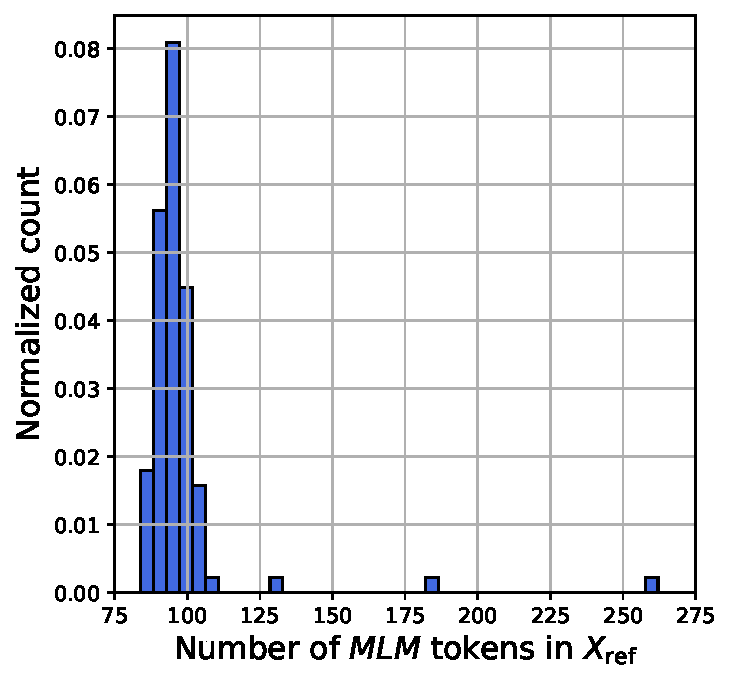
\includegraphics[width=0.35\linewidth]{figures/MLM_tokens.pdf}
}
\subfigure{
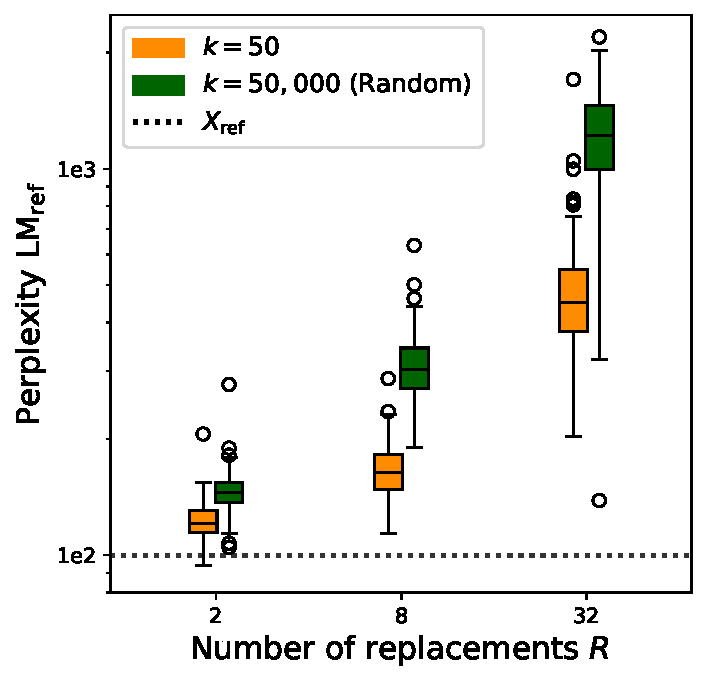
\includegraphics[width=0.35\linewidth]{figures/llama_ppl_neardupls.pdf}
}
\caption{\textbf{Characterizing fuzzy trap sequences.} (a) The distribution of number of tokens $|T_{\text{MLM}}(X_{\text{ref}})|$ of $100$ reference trap sequences. (b) The perplexity computed using $\textit{LM}_{\text{ref}}$ each for $100$ fuzzy trap sequences for token replacement strategies for different values of $k$ across values for $R$.} 
\label{fig:tokens_ppl}
\end{figure*} 

\end{document}